\documentclass{article}
\usepackage{enumitem}
\usepackage{amsmath}
\usepackage[margin=1in]{geometry}
\usepackage{fancyhdr}
\usepackage{graphicx}

\pagestyle{fancy}
\fancyhf{}
\rhead{CS535, Fall 16}
\lhead{Lixuan Zhu (lz306)}
\rfoot{Page \thepage}
\begin{document}
\section{Problem 1}
\begin{enumerate}
\item
    In order for $\Sigma$ to be a valid covariance matrix, $\Sigma$ has to be positive semi-definite. Since a reproducing kernel of a reproducing kernel Hibert space(RKHS) is a positive definite kernel, I first prove that $\sigma(x,x^{'})$ is a such kernel using Fourier transform. According to the definition, RKHS is a Hibert space $H$ consisting of functions on a set $X$ such that for all $x \in X$ there is a function $g_x \in H$ such that $\langle f, g_x\rangle_H = f(x)$, function $g$ being the reproducing kernel of $H$. When realizing RKHS by Fourier transform, we have: $X = R$, $G = L^{2}(R, \rho(t)dt)$ and $J(t;x) = e^{-\sqrt{-1}xt}$. Since the Fourier image of $exp(|x-y|)$ is $\frac{1}{2\pi (t^2+1)}$, let $\rho(t) = \frac{1}{2\pi} \frac{1}{t^2 + \frac{1}{l^2}}$, we have:
    \begin{equation}
    \begin{split}
        k(x,y) &= \frac{1}{2\pi}\int e^{\sqrt{-1}(x-y)t}\frac{1}{t^2 + \frac{1}{l^2}dt}\\
               &= \frac{l}{2}exp(-|x-y|/l) = \frac{l}{2}\sigma(x, y)\\
        H &= \{f\in L^2(R, dx)|\int |f(t)|^2(t^2 + \frac{1}{l^2})dt < \infty\}
    \end{split}
    \end{equation}
Thus $\sigma(x, x^{'})$ is a reproducing kernel of RKHS. According to the definition of positive definite kernel, the matrix $M_{ij} = \sigma(x_i, x_j)$ generatd by $\sigma$ is positive semi-definite. Since $\Sigma$ is such a matrix generated by $\sigma$, it is indeed positive semi-definite and thus a valid covariance matrix.
\item
\item
    According to the definition of statistical correlation:
    \begin{equation}
    \begin{split}
        \rho(y_i, y_j) &= \frac{\sigma(y_i, y_j)}{\sqrt{\Sigma^{y}_{ii}\Sigma^{y}_{jj}}}\\
                       &= \frac{exp(-|y_i - y_j|/l)}{\sqrt{\sigma(y_i, y_i)\sigma(y_j, y_j)}}\\
                       &= \frac{exp(-|y_i, y_j|/l)}{\sqrt{1*1}}\\
        &= exp(-|y_i, y_j|/l)
    \end{split}
    \end{equation}
\item
\item
\item
\end{enumerate}
\section{Problem 2}
\begin{enumerate}
\item
    N/A
\item
    Maximize $log det\Theta - tr(S\Theta)$ subject to $||\Theta||_1 < t$, where $t > 0$ is a tuning factor.
\item
\item
\item
    The adjacency matrix $A$ and precision matrix $\Lambda$ are exactly the same except the diagonal of $A$ is consists of all $0$s while the diagonal of $\Lambda$ is consists of all $1$s. They are both sparse because $Pr(a_{ij} = 1)$ is relativly small thus most of the entries are $0$s. Thus the resulting adjacency graph is also sparse, in some cases some points are disconnected from all other points subject to initial samplingi, as can be observed from Figure 1. In contrast, the covariance matrix $\Sigma_0 = \Lambda_0^{-1}$ is relatively dense, as can be observed from the left most matrix in Figure 1.
    \begin{figure}[h]
        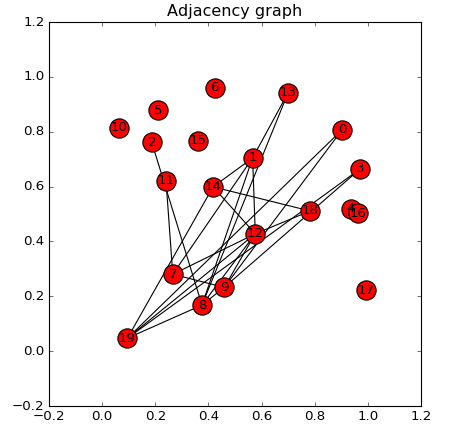
\includegraphics[width=.6\linewidth]{adj.png}
        \caption{Adjacency graph of matrix $A$.}
    \end{figure}
    \begin{figure}[h]
        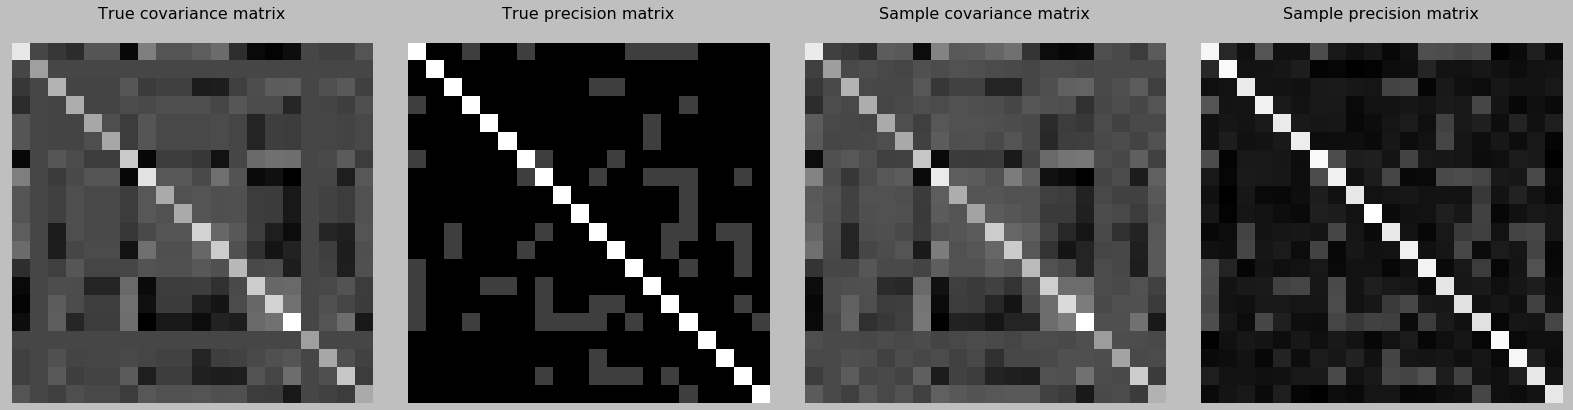
\includegraphics[width=1.15\linewidth]{true.png}
        \caption{"True" covariance/precision matrix and sample covariance/precision matrix.}
    \end{figure}
\item
    According to the sample covariance and precision in the right two matrices of Figure 2, the sample covariance is almost identical to "true" covariance matrix converted from true precision with slight differences since the sample covariance is estimated directly from the dataset. However, the sample precision matrix is much denser than "true" precision matrix because it is computed as the inverse of sample covariance. Slight difference between sample covariance and "true" covariance makes it impossible to reproduce the "true" precision matrix from sample covariance but it is easy to identify the 1 entries in "true" precision matrix from the sample precision matrix although the areas around those entries are blurry (with small non-zero entries).
\item
    \begin{figure}[h]
        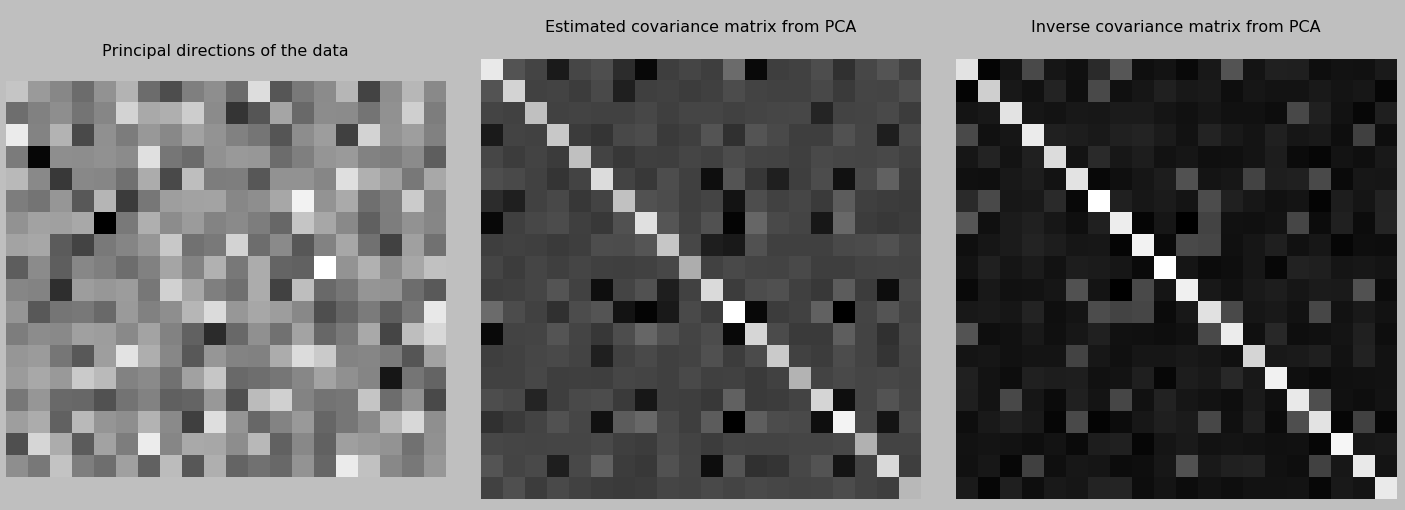
\includegraphics[width=1.1\linewidth]{prin.png}
        \caption{Principle directions and covariance/precision matrix of PCA.}
    \end{figure}
    \begin{figure}[h]
        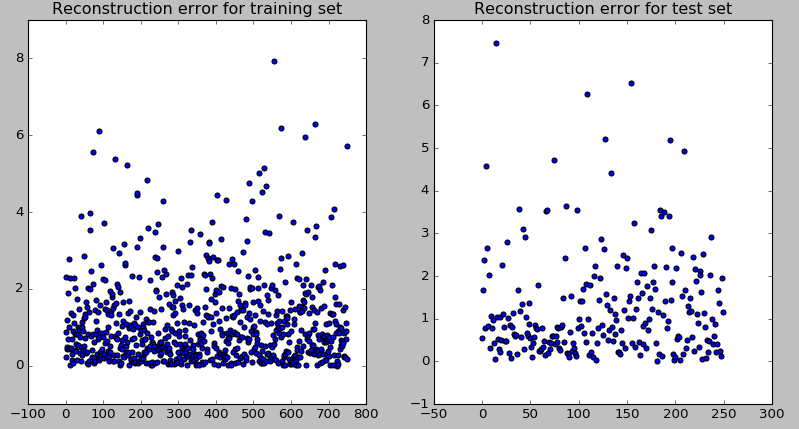
\includegraphics[width=.8\linewidth]{recon.png}
        \caption{Reconstruction errors of training/test sets.}
    \end{figure}
\item
\item
    The Graphical Lasso method estimates a sparse inverse covariance matrix by maximizing the Gaussian log-likelihood of the data. It controls the number of zeros (sparsity) in the inverse covariance matrix by imposing a $L_1$ (lasso) penalty. The algorithm finds the inverse covariance matrix by solving a lasso problem with coordinate descent procedure in each iteration until the resulting matrix converges. Graphical Lasso is much faster compared to other algorithms that solves the same problem.
    \par
    The reconstructed adjacency and covariance matrix are depicted in Figure 6.
    \begin{figure}[h]
        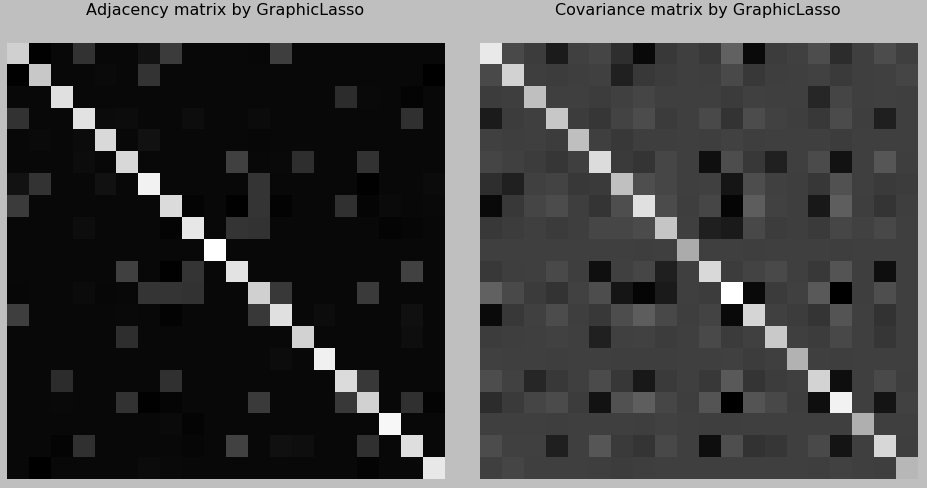
\includegraphics[width=1.0\linewidth]{lasso.png}
        \caption{Adjacency and covariance matrices estimated by Graphical Lasso.}
    \end{figure}
\item
\end{enumerate}
\end{document}
